\documentclass{sig-alternate}

\usepackage{verbatim}
\usepackage{graphicx}
\usepackage{subfig}
\usepackage{algorithmic}

\DeclareCaptionType{copyrightbox}

%define RT-DataPath %BlahSys%

\title{RT-DataPath: Predictable I/O Performance for\\ Push-based Query Processing
Systems}

\numberofauthors{1}
\author{authors}
\toappear{}

\begin{document}

\maketitle

\begin{abstract}
We consider the problem of providing predictable performance for an
application-level workload consisting of many individual queries with specific
response time latency targets. At a low-level we use existing techniques that
provide predictable I/O performance, and avoid worst-case analysis by (1)
extracting performance requirements from the application workload, (2)
transforming these requirements onto the interface of the predictable I/O
sub-system, and (3) intelligently scheduling I/O for efficiency.
\end{abstract}

\section{Introduction}
\label{sec:intro}

%Scientific data volumes are becoming large enough that amortizing the cost of
%storing, managing, and analyzing this data across multiple user groups is
%becoming attractive. Such a system must provide cost effective storage and
%analysis, including the ability to enforce per-user group policies (e.g.
%performance guarantees) in the shared environment.

A new class of science---big data science---is becoming increasingly common
and ever more important. This form of science is characterized by
unprecedented data volume and analysis requirements, an example of which is
the Large Synoptic Survey Telescope (LSST), that in 2018 will begin scanning
the night sky, capturing many petabytes of raw image data over its 10 year
lifespan~\cite{ivezic:arxiv11}. From the raw data collected each night, an
equally voluminous set of meta-data will be extracted, and interestingly,
nearly all of the new science enabled by the LSST will be based on analysis of
this meta-data catalog---stored as a multi-trillion row relational database.
Unfortunately the cost to maintain a dedicated copy of a database this size
will be far beyond the reaches of the vast majority of institutions. What is
needed is a shared system across which a wide range of user groups can
amortize the costs associated with providing broad access to massive data sets
and analysis resources necessary for scientific discovery. The major challenge
of such a system will be providing predictable performance to a broad range of
users while remaining cost effective at high levels of concurrency.
RT-DataPath (RT-DP) addresses this need by combining a new query processing
architecture designed to efficiently support high throughput workloads, with
techniques for guaranteed low-level I/O performance, which together allow the
system to provide predictable query response latencies.

A major obstacle to achieving efficiency \emph{and} predictable response times
in database systems is the use of best-effort data structures and scheduling
semantics. For example complex execution plans compete against each other to
form unattractive I/O access patterns that ultimately lead to resource
contention and degraded, unpredictable performance. A promising approach to
increasing the efficiency and high-concurrency throughput of database systems
is to use a technique called push-based query processing (shared table-scans).
This approach uses a single, unified physical execution plan in which multiple
queries explicitly coordinate to share I/O costs by attaching to a single
stream that sequentially scans an on-disk relation.  Coincidentally, shared
table scans significantly reduce the complexity of providing predictable I/O
performance: all I/O takes the form of sequential scans with required
throughputs, and for any workload, the set of scans can be determined a
priori, allowing admission control and latency prediction for a range of
timeliness guarantees.

\begin{comment}
Previous work~\ref{fahhrad} has shown how hard guarantees can be made for I/O
performance. This work takes the approach that bandwidth cannot effectively be
divided, and that instead the time a disk spends reading data is the only
controllable resource. As a result the expression of application requirements
takes the form of deadlines---time intervals specified by a
\emph{period}---and utilizations per period given by a \emph{rate}.
Unfortunately it is not always simple to determine an appropriate rate and
period to assign to a stream, especially for complex workloads presented by
database systems. We take a simple approach to solving this problem that
involves extracting scan bandwidth requirements from a query workload, and
only admitting new queries if they do not cause existing performance
guarantees to be violated\footnote{It is possible for a query to always be
admitted with best-effort, and starvation prevention policies, but we focus in
this paper on the problem of hard guarantees.}.

When each query in a workload depends on a single scan this approach works
well---each scan requires a specific bandwidth which is either feasible or
not.  However, queries that contain multi-stage operators may depend on
multiple scans with inter-dependencies. For example, a JOIN may first scan the
RHS table to build a hash-table, and only afterwards scan the LHS table to
probe the index. A simple approach to forming I/O reservations is to
over-provision assuming that \emph{all} scans run concurrently, but this may
artificially limit the available I/O bandwidth that would otherwise be
available to admit additional queries into the system. Our system addresses
this concern by taking into account operator implementation (e.g. hash-join)
when calculating I/O reservations.  Specifically, we transform a query
workload into a series-parallel partial ordering of scans that describes the
inter-dependencies between scans of the workload, allowing us to dynamically
adjust I/O reservations and avoid over-provisioning for worst-case analysis.

Increasing performance and efficiency for shared scientific data warehouses
will become essential to productive (and cost effective) science. Work and
data sharing is one way to handle the massive levels of concurrency that will
exist as the number of users interacting with the system increase, but
integrating performance guarantees into a complex system is difficult. Our
system introduces techniques for achieving both efficient execution and
performance guarantees.
\end{comment}

This paper makes the following contributions.

\begin{enumerate}
\item WIP
\begin{comment}
\item We utilize existing technologies (Fahrrad) to provide performance
isolation and predictability at the lowest-level (disks), and introduce
high-level scheduling techniques to manage competition between application IO
streams.
\item We draw inspiration from CPU scheduling treating IO streams as
\emph{tasks}, and disks and flash devices as \emph{CPUs}.
\item Description of the higher level part of the system: push-based
approach...  (we will add some description later).
\item There should be a simple example that demonstrates the problem. One
possibility is to show an example in which several streams cannot meet their
deadlines when run concurrently, but can when they are intelligently scheduled
at a higher level.
\end{comment}
\end{enumerate}

\section{Overview of RT-DataPath}
\label{sec:overview}

RT-DataPath provides predictable I/O performance for relational query
workloads. The architecture of RT-DP is illustrated at a high-level in
Figure~\ref{fig:sysarch}, and consists of three components that work together
to evaluate queries with associated response time latencies. First, query
processing in RT-DP uses DataPath, a push-based execution engine that can
efficiently support high-concurrency workloads. At a low-level, predictable
I/O performance is provided by (Fahrrad, Qbox, ..), a system that enforces
application performance reservations. Finally, RT-DP analyzes high-level query
workloads, translating their performance requirements into the low-level
specifications required by the storage QoS layer.

When a query is submitted by an application the system determines if it can be
evaluated without violating existing performance guarantees by verifying that
the total I/O utilization of the new workload is less than $100\%$. Rejected
queries can be reported with latency estimates and provisionally accepted with
soft or best-effort guarantees.

\subsection{Application Workload}

We consider an application workload to consist of a set of queries $W$, where
each query $q \in W$ has an associated latency $L_q$ that specifies an upper
bound on when the system must return the result of evaluating $q$ to the
application that submitted the query. We currently consider workloads without
updates which will be common for large scientific data warehouses with
periodic bulk updates.  As a notational convenience we allow a group of
queries $G \subseteq W$ to have a common latency $L_G$, in which case all
queries $q \in G$ have latency $L_q = L_G$. This is useful for applications
that want to construct a set of queries that should finish at the same time.

\subsection{Query Processing in DataPath}
\label{sec:push}

Query processing in RT-DataPath uses DataPath, a push-based database system in
which shared-table scans feed data into a single, unified physical execution
plan. In this paper we present the salient features of DataPath most relevant
to RT-DataPath, and direct the reader to a detailed discussion of the system
found in ~\cite{arumugam:sigmod10}. Consider now the following workload
consisting of the three queries:\\

\noindent
$Q_1$: \texttt{SELECT AVG(o\_temperature) FROM Object\\
WHERE o\_date < '1-1-10';}\\

\noindent
$Q_2$: \texttt{SELECT AVG(o\_humidity) FROM Object\\
WHERE o\_date < '1-1-99';}\\

\noindent
$Q_3$: \texttt{SELECT COUNT(*) FROM Object, Location\\
WHERE l\_elevation < 10 AND o\_lid = l\_lid;}\\
\\
{\bf Query evaluation.} The DataPath system evaluates these three queries by
first forming a single physical execution plan for the entire workload,
structured as a directed acyclic graph (DAG), and shown in
Figure~\ref{fig:datapath_dag}. The directed paths in the DAG correspond to the
flow of tuples, and each node represents an operator in the plan. To
illustrate how the DAG is used to evaluate the workload we begin by
considering the execution of query $Q_1$. At the lowest level a scan over the
\emph{Object} relation is initialized, and all tuples in the relation are
pushed into the first node which applies the predicate \texttt{o\_date <
'1-1-10'}. Next, each matching tuple is pushed into the next upstream node
that implements the \texttt{AVG} operator. Once the entire table has been
scanned, and the DAG has processed each tuple, the final result can be
produced.

\begin{figure}[ht]
\centering
\subfloat[] {
 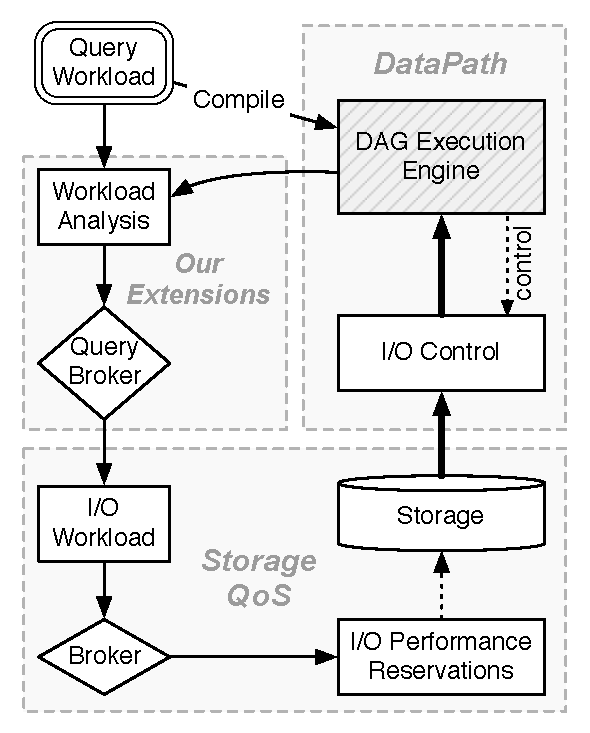
\includegraphics[scale=0.4]{fig-overview}
 \label{fig:sysarch}
} 
\subfloat[] {
 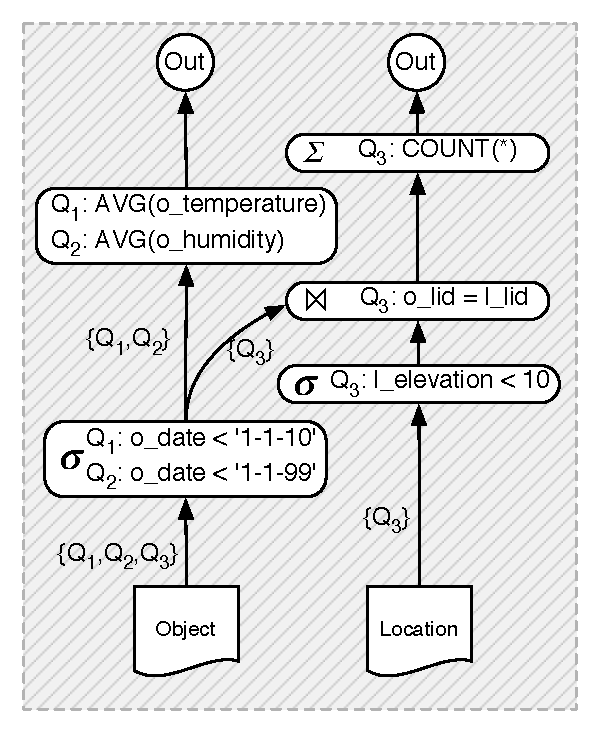
\includegraphics[scale=0.4]{fig-dag}
 \label{fig:datapath_dag}
}
\caption{(a) high-level architectural view of RT-DataPath. (b) physical
execution plan for queries $Q_1$, $Q_2$, and $Q_3$, structured as a directed
acyclic graph.\\}
\end{figure}

{\bf Work sharing.} Consider now the concurrent evaluation of queries $Q_1$
and $Q_2$, again shown in Figure~\ref{fig:datapath_dag}. Each query computes
the average of a distinct attribute from the \texttt{Object} relation, applies
a selection predicate to the \texttt{o\_date} field, and most importantly,
each query can be evaluated by sharing the stream of tuples produced by the
\emph{single} scan over the \texttt{Object} table---meaning that the costly
I/O required to read tuples need only be incurred once---shared across all
queries depending on a scan over the relation.  This type of I/O optimization
is simply not practical in a traditional iterator-based architecture as all
sharing would need to be coordinated through the buffer-cache across
independently executing physical plans. However, this unchecked competition
between execution plans results in the type of induced random I/O that limits
system throughput.

{\bf Join processing.} Finally we examine how query $Q_3$ is evaluated, and in
particular how join processing is handled.  DataPath uses a hash-join
algorithm that is composed of two execution stages.  In the first stage a hash
table is built over the right-hand-side relation, and in the second stage the
hash table is probed with tuples from the left-hand-side relation. Thus the
system executes $Q_3$ by first scanning the \texttt{Location} relation to
construct a hash table, after which the \texttt{Object} relation is scanned
and the hash table probed for matches. Observe that work sharing now occurs
across the entire workload: queries $Q_1$, $Q_2$, and the second stage of
$Q_3$, all share the I/O cost of scanning the \texttt{Object} relation.

{\bf Predictable execution latency.} The cost of performing I/O in a
data-intensive system can account for a significant fraction of total query
execution time, and thus unpredictable I/O performance can have a direct
impact on the predictability of query execution time. In
Section~\ref{sec:ioqos} we present an existing solution to providing storage
QoS, and in Section~\ref{ioqosdp} we show how RT-DataPath bridges the gap
between DataPath's I/O system and an underlying storage QoS system to increase
total run-time predictability.

\subsection{Storage I/O Quality-of-Service}
\label{sec:ioqos}

DataPath is designed to maximize I/O throughput by striping data across many
disks, and unfortunately it does not provide the ability to enforce specific
QoS requirements on its low-level I/O streams. RT-DataPath bridges the gap
between DataPath and existing solutions that provide storage QoS, by analyzing
a query workload and its associated physical execution plan to derive specific
performance requirements for the low-level I/O streams that implement each
table scan. In general it is a difficult problem to virtualize the performance
of storage devices and there are many solutions with different trade-offs. We
have chosen to use one existing solution, (Fahrrad, Horizon, or Qbox), which
provides, WIP.

{\bf Interface.} The interface is straight forward for the discussion of
RT-DataPath. It is a workload specification for a particular I/O stream that
includes information about throughput and latency, timeliness requirements,
and workload behavior (sequential, random). This high-level description of the
performance requirements is used internally to make reservations. This
translation is performed by a component called the broker.

{\bf Admission control.} Admission control accepts new reservations only if
all existing guarantees can still be met, otherwise the reservation is
rejected. Rejected workloads can be augmented with alternative QoS
requirements that could be met, or accepted with best-effort semantics.\\\\

\subsection{Predictable I/O Performance in DataPath}
\label{sec:ioqosdp}

{\bf The basics.} A table scan is the basic unit of I/O used in DataPath to
process a query. Thus, given a relation $T$, its on-disk size $|T|$, and a
target response time latency $L_q$, it is straight-forward to calculate the
required rate at which data must be delivered to the execution engine as
$|T|/L_q$ in order to meet the response deadline. When multiple queries depend
on a table scan, the bandwidth requirement of the associated I/O stream is
calculated based on the query with the smallest response time latency.

{\bf Multi-scan operators.} Queries that depend on multiple table scans, such
as those using a hash-join implementation (see \S\ref{sec:dpqe}), complicate
the calculation of per-table I/O throughput because the requested latencies
must be divided into sub-latencies and assigned to each individual scan. One
simple approach is to assign sub-latencies proportional to the size of the
relation. For example, a query with latency $L_q$ that must scan $T_1$ and
then $T_2$ could use a bandwidth requirement of $(|T_1| + |T_2|)/L_q$ for each
scan. In general there are many policies by which latencies can be
sub-divided. RT-DataPath explores the trade-offs of various heuristics.

{\bf Over-provisioning.} RT-DataPath splits query latencies across scans when
multi-scan operators are used in a physical execution plan.  However, there
often exists a serial dependency between scans for a particular query---scan
right-hand-side relation \emph{then} scan the left-hand-side relation. If
bandwidth reservations are made assuming all scans run concurrently then
over-provisioning can occur, artificially inflating the required throughput of
the storage system and reducing the flexibility of the system.  RT-DataPath
avoids bandwidth over-provisioning by exploring the state space of scan
combinations to ensure that workload feasibility is only verified for
\emph{valid} scenarios.

\section{Preliminaries}

{\bf Assumptions.} We assume a single node, single disk setup and a read-only
workload. Probably there are some other things, too. There are a set $\{T\}$
of tables in the system without duplicates. There is a single I/O stream scan
per table.

{\bf DataPath interface.} DataPath takes as input the query workload $W$ and
produces a physical execution plan $DAG(W)$ (illustrated in Figure~\ref{}). We
assume that $DAG(W)$ exposes several properties about the execution plan that
are available to RT-DataPath:

\begin{enumerate}
\item Let $Q_T \subseteq W$ be the set of queries that depend on a scan over
	table $T$. The set $Q_T$ is empty if no query depends on the relation $T$.
	An example of such a set is illustrated in at the bottom of Figure~\ref{}.
\item For any query $q \in W$ let $T_q$ be the set of tables $T \in T_q \iff q
	\in Q_T$. In other words, it is the set of tables that need to be scanned
	on behalf of query $q$. This set can be derived from $Q_T$.
\item $D(T_q)$ is the set of inter-dependencies between scans of table $T_q$.
	For example, if $q$ is a join query then $DAG(W)$ will expose $D(T_q)$
	that expresses that the LHS relation is scanned after the RHS.  \emph{This
		notation is intentionally vague at the moment as we are not yet sure
	precisely what information needs to be in it}.
\end{enumerate}

{\bf Storage interface.} RT-DataPath assumes the existence of a storage
system~\ref{blah} capable of allowing bandwidth reservations to be made. We
use $B_T$ to denote the bandwidth (MB/s) requirement for the I/O stream
associated with the scan over table $T$.

\section{Workload Analysis}

RT-DataPath uses the workload $W$ and information exposed by the physical
execution plan $DAG(W)$ to calculate, for each table $T$, a bandwidth
reservation $B_T$ to assign to the I/O stream that implements the scan over
the relation $T$. For any table $T$ we define $B_T$ to be the minimum
bandwidth needed to meet the QoS requirements of all the queries that depend
on scanning $T$:

\begin{center}
$B_T = \max_{L \in L_T} \frac{|T|}{L}$
\end{center}

\noindent
where $|T|$ is the size of the stored relation and $L_T$ is the set of scan
latencies that need to be ``enforced'' for each query in $Q_T$, the set of
queries depending on scans over $T$.

{\bf Calculating $L_T$.} The set $L_T$ is constructed by calculating the
latencies ``contributed'' by each query that depend on a scan of table $T$.
The required latency to scan $T$ on behalf of a query $q \in Q_T$ is given as
$L^q_T \in L_T$, a fraction of its total application-specified latency budget
$L_q$. The simplest case occurs when $|T_q| = 1$, that is, $q$ depends on a
scan of exactly one table where $L^q_T = L_q$.

When $|T_q| > 1$ a query's total latency budget $L_q$ must be divided/split
between the table scans of $T_q$. Given a policy $P$ and $D(T_q)$, a query
latency $L_q$ is divided between each table $T \in T_q$ into separate
contributed latencies $L^q_T$. In Section~\ref{sec:latsplit} we discuss
latency splitting policies.

\subsection{Latency Splitting Policies}

There may be multiple policies here. Once simple policy is to split the
latencies proportional to the size of the relations being scanned. Another
policy might incorporate some slack to account for the cost of switching
scans.

\section{Binary Integer Program}

\[
\sum_{n \in [0,|Q|]} \sum_{q,t \in Q} s_{qn} (t - t_S(q,n)) + i_{qn} (t -
t_I(q,n)) + is_{qn} (t - t_{IS}(q,n))
\]

\[
z_n = 1 \iff s_{qn} \vee i_{qn} \vee is_{qn}
\]

\[
s_{qn} + i_{qn} + is_{qn} \le 1, \forall q \in Q
\]

\[
\sum_{n \in [0, |Q|]} i_{qn} + is_{qn} + s_{qn} = 1, \forall q \in Q
\]

\[
z_n \ge i_{qn} + is_{qn} + s_{qn}, \forall n \in [0, |Q|]
\]

\[
\sum_{n \in [0, |Q|]} z_n = 1
\]

\section{Broker and Admission Control}

The purpose of the broker is to use the bandwidth requirements computed during
the workload analysis phase and determine if the storage QoS system can
support the workload. The storage QoS system either accepts or rejects the
workload's bandwidth requirements. There are two scenarios. The first is that
the workload contains no multi-stage queries and thus there is only one
combination of scans that must be checked. However, if multi-stage queries are
in the workload there are more than one possible scan combinations to check.

{\bf Illustrative example.} The previous workload shown in Section 2 has three
queries. Queries $Q_1$ and $Q_2$ and the second stage of $Q_3$ depend on table
$T_1$, and the first stage of $Q_3$ depends on table $T_2$. After workload
analysis there will be some bandwidth needed for $T_1$ and some bandwidth
needed for $T_2$. However, the only possible run-time scenarios are $\{Q_1,
Q_2, Q_3'\}$ \emph{or} $\{Q_1, Q_2, Q_3''\}$ where $Q_3', Q_3''$ are the first
and second stages, respectively. To avoid over provisioning we do not want to
reserve bandwidth for both stages of $Q_3$ running concurrently, but we
simultaneously must ensure that each scenario is feasible.

In the worst case we must ask the storage broker if all of the combinations in
the state spaces are possible. In the best case this state space can be
reduced to a single question (most likely), or some heuristic is needed to
trim the space.

\bibliographystyle{plain}
\bibliography{refs}

\end{document}
